\documentclass[10pt, final, hyperref, table]{beamer}
\mode<presentation>


 %\usepackage[english]{babel} % "babel.sty"
% \usepackage{french}                  % "french.sty"
%  \usepackage{franglais}               % "franglais.sty" (a defaut)
  \usepackage{times}            % ajout times le 30 mai 2003
 
%% --------------------------------------------------------------
%% CODAGE DE POLICES ?
%% Si votre moteur Latex est francise, il est conseille
%% d'utiliser le codage de police T1 pour faciliter la césure,
%% si vous disposez de ces polices (DC/EC)
\usepackage[utf8]{inputenc}
\usepackage[T1]{fontenc}
\usepackage{eurosym}


%% ==============================================================
%\usepackage{graphicx}
\usepackage{amsmath,amsfonts}
%\usepackage[table]{xcolor}
\usepackage{subfigure}
\usepackage{fancybox}

\usepackage{multicol}
\usepackage{wrapfig}
\usepackage{listings}
\usepackage{xcolor}
\usepackage{multimedia} % For playing sound

\usepackage{hyperref}
% Define hyperlinks color
\definecolor{links}{HTML}{2A1B81}
\hypersetup{colorlinks,linkcolor=,urlcolor=links}

\usetheme{Madrid}
\setbeamercovered{transparent}


% telemeta red
\definecolor{telemetaRed}{rgb}{0.41568, 0.01176, 0.02745}   % #6A0307
\usecolortheme[rgb={0.41568, 0.01176, 0.02745}]{structure} 

%\setbeamercolor{frametitle}{bg=telemetaRed}
% Display a grid to help align images
%\beamertemplategridbackground[1cm]

%We will get the normal bibliography style (number or text instead of icon) by including the following code
\setbeamertemplate{bibliography item}[text]
\setbeamerfont{caption}{size=\footnotesize}
% listings settings
\definecolor{lstComments}{rgb}{0,0.6,0}
\definecolor{lstBkgrd}{rgb}{0.95,0.95,1}
\lstset{%
  language=Python, % the language of the code
  frame=single,  % adds a frame around the code
  frameround=tttt,
  commentstyle=\color{lstComments},% comment style
  backgroundcolor=\color{lstBkgrd},   % choose the background color
  basicstyle=\tiny,       % the size of the fonts that are used for the code
  stringstyle=\ttfamily,  % typewriter type for strings
  keywordstyle=\color{blue},      % keyword style
  showstringspaces=false,          % underline spaces within strings only
}


\definecolor{rouge}{rgb}{1.0,0,0}
\newcommand{\chref}[2]{
    \href{#1}{\color{rouge}\underline{#2}}
}
\newcommand{\dchref}[1]{
    \href{#1}{\color{rouge}\underline{#1}}
}
\newcommand{\curl}[1]{
    \color{rouge}\underline{\url{#1}}
}
\title[Telemeta]{Telemeta\\ open web audio content management system}

\author{Guillaume Pellerin\inst{1}}

\institute[Parisson]{
  \inst{1}%
  Parisson, Paris, France\\
\vskip1ex
 \begin{center}
   \includegraphics[width=.3\linewidth]{img/parisson_logo_FINALE_com.pdf}
 \end{center}
}

\date[DML 1st Workshop - 19/03/2014]{Digital Music Lab 1st Workshop - 19/03/2014}        

\begin{document}
\frame{\titlepage}


\section[Table of contents]{}
\frame{\frametitle{Table of contents}
\tableofcontents
}

\section{Goals}
\frame{\frametitle{Main goals}
\vspace{-1cm}
\center{\includegraphics[width=4cm]{img/logo_telemeta_1-1.pdf}}
\vspace{0.5cm}
\begin{itemize}
  \item \alert{Save}, \alert{scale} and \alert{sustain} big music data and related metadata
  \item \alert{Play} audio and read metadata \alert{synchronously}
  \item \alert{Index} and \alert{share} music data through a \alert{collaborative} web app
  \item \alert{Link} music data to various \alert{ontologies} and \alert{external services}
  \item \alert{Manage} \alert{workflow} rules (access, copyrights) easily through time
  \item \alert{Process} audio \alert{on demand} through a \alert{modular architecture}
\end{itemize}
}

\section{History}
\frame{\frametitle{History of the project}
\begin{itemize}
  \item \alert{2006} : definition of the goals (open source web audio collaborative platform)
  \item \alert{2007} : first partner : CREM
  \item \alert{2007 - 2009} : technical specifications, definition of the DB migrator
  \item \alert{2008} : prototype development
  \item \alert{2008 - 2010} : workflow and format specifications 
  \item \alert{2011} : development, final migration and release of \alert{Telemeta 1.0} to the CREM for production : \dchref{http://archives.crem-cnrs.fr}
  \item \alert{2011 - 2014} : collaborative indexing, more development, massive data imports...
\end{itemize}
}

\section{Technologies}
\frame{\frametitle{Technologies}
\begin{center}
\large{\alert{100\% 0pen Source!}}
\end{center}

\begin{itemize}
 \item \chref{http://python.org}{Python} : smart object oriented language \\
 \item \chref{http://djangoproject.com}{Django} : high-level web MVC framework \\
 \item \chref{https://github.com/yomguy/TimeSide}{TimeSide} : open web audio processing framework 
 \item \chref{http://gstreamer.freedesktop.org/}{GStreamer} : open source multimedia framework
 \item MySQL, PostgreSQL, others : relational databases \\
 \item GNU / Linux : applications, libraries and kernel \\
\end{itemize}
}

\section{Features}
%\frame{\tableofcontents[currentsection]}
\frame{\frametitle{Key features}
      \begin{itemize}
      \item \alert{Pure HTML5} web user interface including dynamical forms
        and smart workflows
      \item \alert{On the fly} audio analyzing, transcoding and metadata
        embedding in various formats
      \item \alert{Social editing} with \alert{semantic ontologies}, smart workflows,
        realtime tools, human or automatic \alert{annotations and
        segmentations}
      \item \alert{User management} with individual desk, playlists, profiles
        and access rights
      \item \alert{High level search engine} (geolocation, instruments, ethnic groups, etc...)
      \item \alert{Data providers} : DublinCore, OAI-PMH, RSS, XML, JSON and other 
      \item \alert{Multi-language} support (now english and french)
      \end{itemize}
}


\section{Architecture}
\frame{\frametitle{Architecture}
    \begin{center}
    \pgfimage[width=8cm]{img/TM_arch}
    \end{center}
}

\section{Data model}
%\frame{\tableofcontents[currentsection]}
\frame{\frametitle{Data model}
\begin{itemize}
 \item Main resource objects
    \begin{center}
    \pgfimage[width=10cm]{img/TM_model}
    \end{center}
 \item Complete model : \chref{http://telemeta.org/export/cb1fc9ad29e2cb0122fde9dd76c5275ba5dc7d14/doc/devel/telemeta-all.pdf}{view PDF}
\end{itemize}
}


\section{Workflow}
\frame{\frametitle{Workflow}
    \begin{center}
    \pgfimage[width=12cm]{img/TM_workflow}
    \end{center}
}

\section{Web interface}
\begin{frame}\frametitle{Web interface}
  \vspace{-0.25cm}
  \begin{center}
    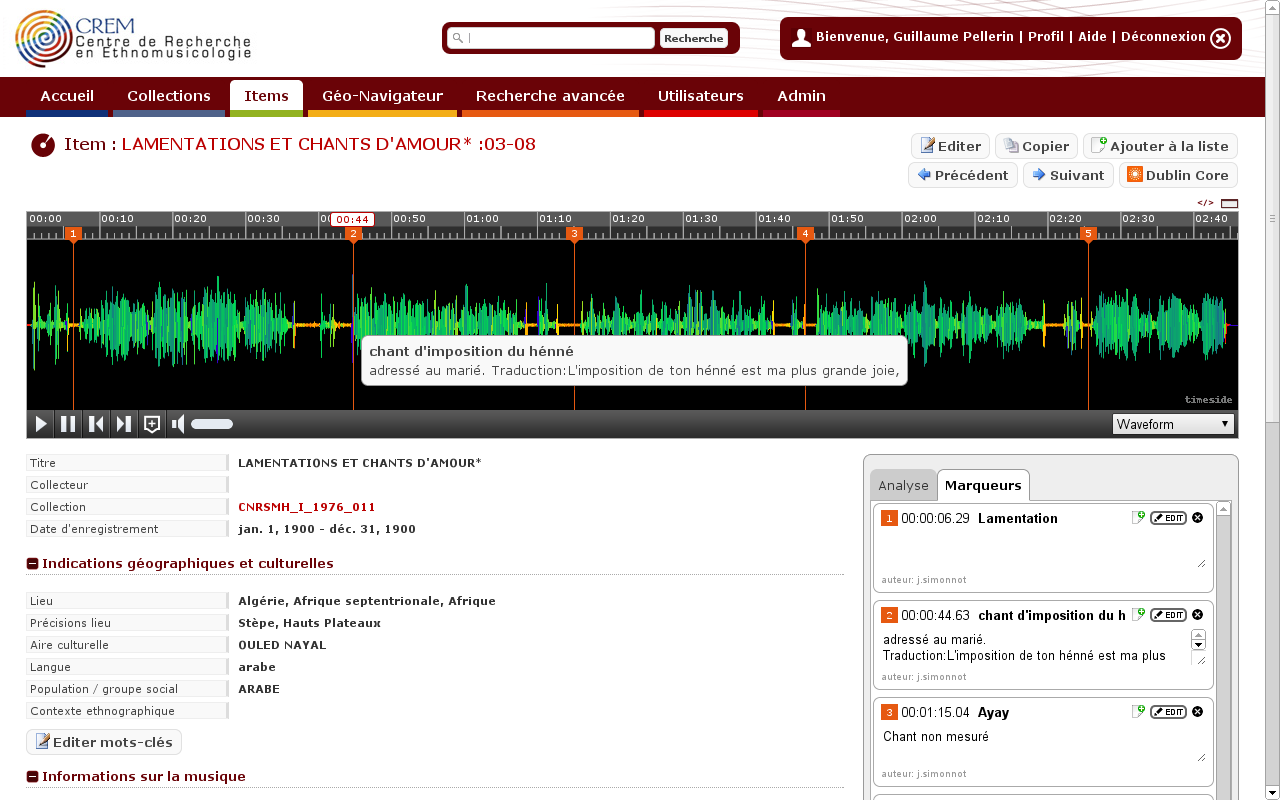
\includegraphics[width=12cm]{img/shots/player_mark.png}
  \end{center}
  \tiny{\url{http://archives.crem-cnrs.fr/archives/items/CNRSMH_I_1976_011_003_08/}}
\end{frame}


\section{Related projects}
\frame{\tableofcontents[currentsection]}

\begin{frame}
 \frametitle{TimeSide : open web audio processing framework}%\scriptsize
% ==================================
% --------- Résumé -----------------
% ==================================
\begin{block}{Server side - TimeSide Engine}

  \begin{itemize}
  \item \alert{Do} asynchronous and fast audio processing with Python,
  \item \alert{Decode} audio frames from ANY format into numpy arrays,
  \item \alert{Analyze} audio content with state-of-the-art audio feature extraction libraries,
  \item  \alert{Organize}, serialize and save analysis metadata through various formats,
  \item  \alert{Draw} various fancy waveforms, spectrograms and other cool graphers,
  \item  \alert{Transcode} audio data in various media formats and stream them through web apps,

    \end{itemize}
 
\end{block}
\begin{block}{Client side - TimeSide UI}
  \begin{itemize}
  \item   \alert{Playback} and  \alert{interact} on demand through a smart high-level HTML5 extensible player,
  \item   \alert{Index},  \alert{tag} and  \alert{organize semantic metadata} \\
(see \href{http://telemeta.org/}{Telemeta} which embeds TimeSide). 
\hfill $\vcenter{\hbox{\includegraphics[width=0.2\textwidth]{img/logo_telemeta_1-1.pdf}}}$
 % \begin{flushright}
 %   
\includegraphics[width=0.2\textwidth]{../../Common/img/logo_telemeta_1-1.pdf}\\
 %   \colorbox{yellow!50}{\textbf{\url{http://telemeta.org/}}}
  %\end{flushright}
  \end{itemize}
\end{block}
\end{frame}

\begin{frame}
  \frametitle{TimeSide - Architecture}
  \begin{center}
    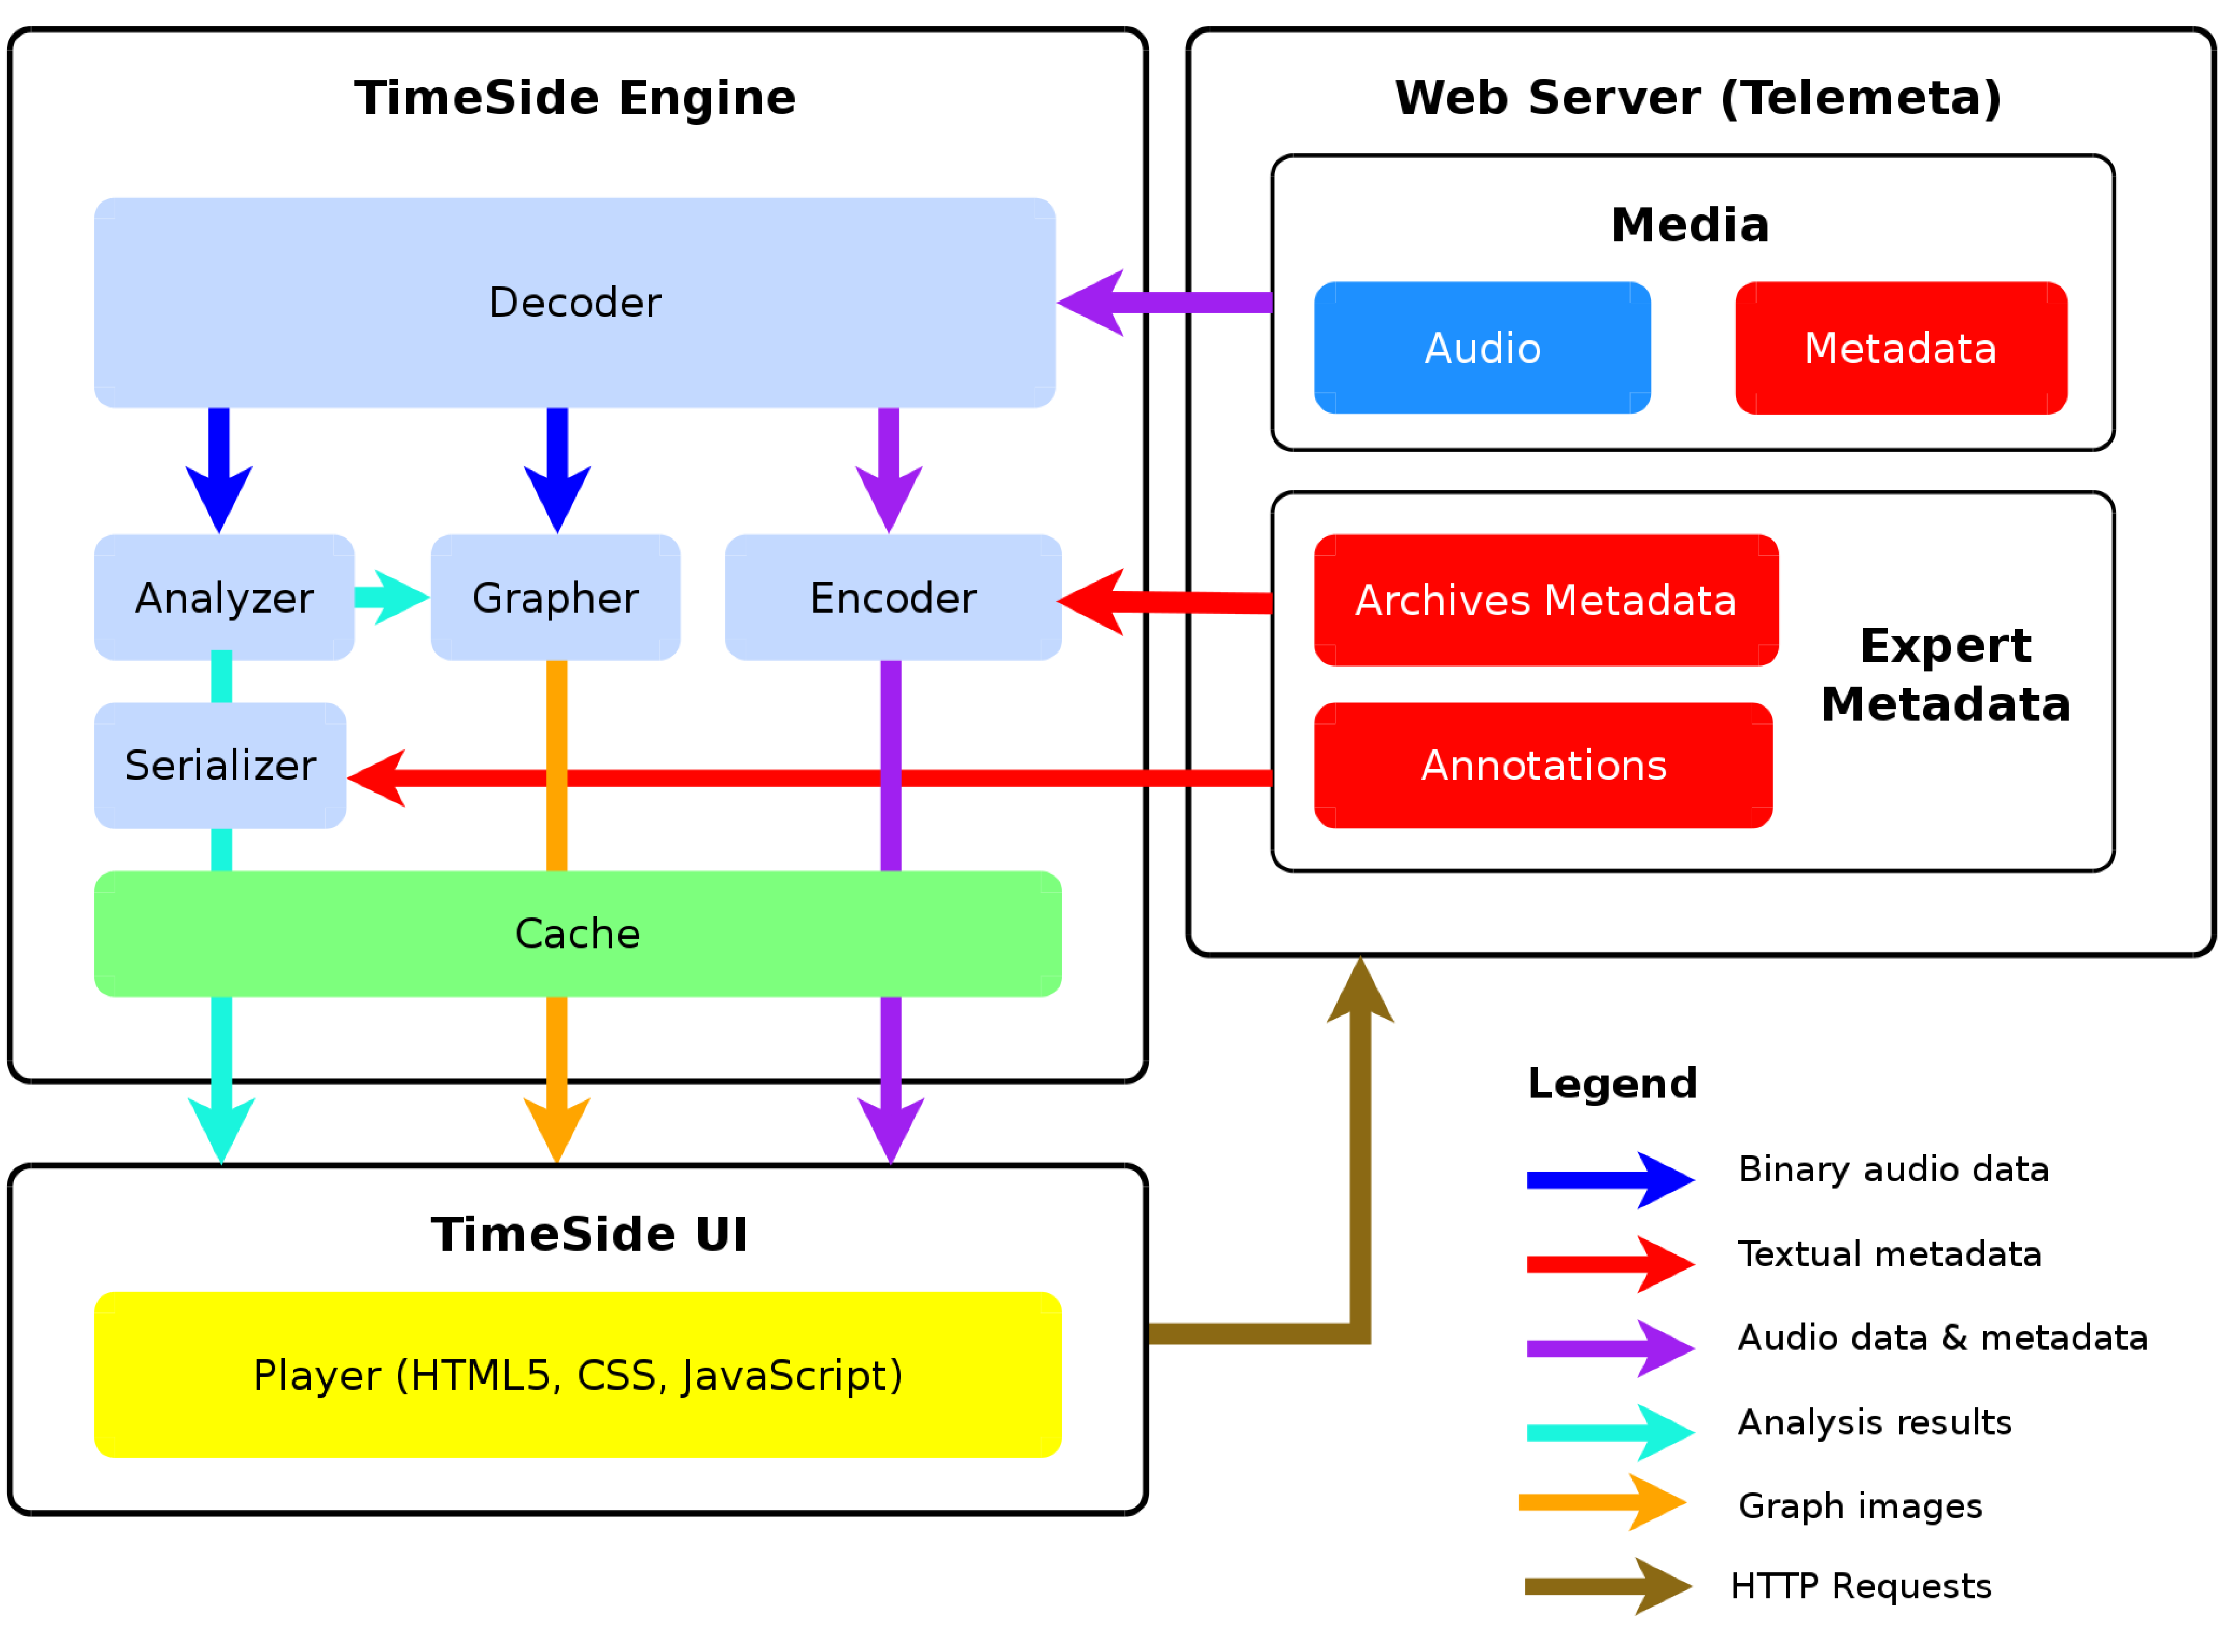
\includegraphics[width=0.8\textwidth]{img/timeside_schema_v3.pdf}
  \end{center}
\end{frame}



\frame{\frametitle{DIADEMS}
\begin{itemize}
    \item \chref{http://www.irit.fr/recherches/SAMOVA/DIADEMS/fr/welcome/&cultureKey=en}{DIADEMS} : Description, Indexation, Access to Sound and Ethnomusicological Documents
    \item granted by ANR : french national research agency (ANR-12-CORD-0022)     
    \item 3 years, 8 partners, 850 k\euro
    \item new collaboration between human and computer science laboratories (not so easy!)
    \item apply and test MIR algorithms on large scale ethnomusicological data
    \item define some high level interfaces to find musical informations in complex corpus
    \item define some \chref{http://files.parisson.com/telemeta/telemeta-doc/DIADEMS/thesaurus/Thesaurus/Thesaurus.html}{thesauri} describing ethnomusicilogy events
    \item \dchref{http://www.irit.fr/recherches/SAMOVA/DIADEMS/fr/welcome/}
    \item \dchref{http://diadems.telemeta.org}
\end{itemize}
}

\frame{\frametitle{DIADEMS - Partners}
\begin{itemize}
\item Sponsors:
\begin{itemize}
 \item CNRS
 \item Huma-Num (ex TGE Adonis)
 \item ANR
 \item CREM
 \item UPMC
 \item Parisson
\end{itemize}

\vspace{0.25cm}

\item Partners :
\begin{itemize}
\item IRIT (université Paul Sabatier, Toulouse 3)
\item LIMSI (universités Pierre et Marie Curie (UPMC, Paris 6) et Paris-Sud)
\item LAM (institut Jean Le Rond d'Alembert, UPMC)
\item LABRI (université de Bordeaux)
\item CREM (université Paris Ouest Nanterre La Défense)
\item LESC (université Paris Ouest Nanterre La Défense)
\item Museum d'Histoire Naturelle de Paris
\item Musée du Quai Branly
\end{itemize}

\end{itemize}

\begin{center}
\begin{columns}[c]
\column{2.5cm}
\begin{center}
\pgfimage[width=1cm]{img/logo-CNRS}\end{center}
\column{2.5cm}
\begin{center}
\pgfimage[width=2.5cm]{img/Logo-CREM-La.jpg}
\end{center}
\column{2.5cm}
\begin{center}
\pgfimage[width=2.5cm]{img/parisson_logo_200}\end{center}
\column{2cm}
\begin{center}
\pgfimage[width=1.2cm]{img/logo-mnhn}\end{center}
\end{columns}
\end{center}

}


\frame{\frametitle{DIADEMS - Roadmap}
\begin{center}
\pgfimage[width=12cm]{img/TM_Roadmap}
\end{center}
}

\frame{\frametitle{TODO list}
\begin{block}{TimeSide}
    \begin{itemize}
    \item web server (django)
    \item process task manager
    \item full HTML5 zooming player (+ annotations, segmentations, etc..)
    \item analyzer parameters (+ interface)
    \item more filtering (FIR, IIR, phase vocoder)
    \item \dchref{https://github.com/yomguy/TimeSide/issues}
    \end{itemize}
\end{block}
\begin{block}{Telemeta}
    \begin{itemize}
    \item class based views
    \item rewrite geolocation services
    \item public and enhanced user playlists
    \item smart breadcrumbs 
    \item better interactions with TimeSide
    \item \dchref{http://telemeta.org/report/1}
    \end{itemize}
\end{block}
}

\section{Development}
%\frame{\tableofcontents[currentsection]}
\frame{\frametitle{Development}
\begin{block}{Links}
    \begin{itemize}
    \item \dchref{http://telemeta.org}
    \item \dchref{https://github.com/yomguy/Telemeta/}
    \item \dchref{https://github.com/yomguy/TimeSide/}
    \end{itemize}
\end{block}
\begin{block}{Team}
    \begin{itemize}
     \item Guillaume Pellerin
     \item Thomas Fillon
     \item Paul Brossier
     \item Riccardo Zaccarelli
     \item Maxime Lecoz
     \item David Doukan
    \end{itemize}
\end{block}
\begin{block}{Licence}
\chref{http://www.cecill.info/licences/Licence_CeCILL_V2.1-en.html}{CeCILL v2.1} (GPL v2 compatible) 
\end{block}
}


\frame{\frametitle{The End}
 \begin{center}
   \large{Thank you!}
   \vspace{0.25cm}
    \begin{block}{Links}
     \begin{itemize}
        \item \chref{http://telemeta.org}{telemeta.org}
        \item \chref{https://twitter.com/telemeta/}{@telemeta}
    \end{itemize}
    \end{block}
    \begin{block}{Me}
    \begin{itemize}
    \item \chref{mailto:guillaume@parisson.com}{guillaume@parisson.com}
    \item \chref{https://twitter.com/yomguy/}{@yomguy}
    \item \chref{https://github.com/yomguy/}{github.com/yomguy/}
    \item \chref{https://plus.google.com/u/0/+GuillaumePellerin/posts}{+GuillaumePellerin}
    \item \chref{http://fr.linkedin.com/in/guillaumepellerin}{fr.linkedin.com/in/guillaumepellerin}
    \end{itemize}
     \end{block}
  \end{center}
}

\end{document}